
\documentclass[landscape,a0b,final]{a0poster}


\usepackage{epsfig}
\usepackage{multicol}
\usepackage{pstricks,pst-grad}
\usepackage{graphicx}
\usepackage{caption}
\usepackage{color}
\usepackage{amsmath}
\usepackage{subcaption}




%%%%%%%%%%%%%%%%%%%%%%%%%%%%%%%%%%%%%%%%%%%
% Definition of some variables and colors
%\renewcommand{\rho}{\varrho}
%\renewcommand{\phi}{\varphi}
\setlength{\columnsep}{2cm}
\setlength{\columnseprule}{0mm}
\setlength{\parindent}{0.0cm}




%%%%%%%%%%%%%%%%%%%%%%%%%%%%%%%%%%%%%%%%%%%%%%%%%%%%%%%%%%%%%%%%%%%%%%
%%% Begin of Document
%%%%%%%%%%%%%%%%%%%%%%%%%%%%%%%%%%%%%%%%%%%%%%%%%%%%%%%%%%%%%%%%%%%%%%

\begin{document}

\vspace*{1cm}


\newrgbcolor{lightblue}{0. 0. 0.80}
\newrgbcolor{white}{1. 1. 1.}
\newrgbcolor{whiteblue}{.80 .80 1.}

%%%%%%%%%%%%%%%%%%%%%
%%% Header
%%%%%%%%%%%%%%%%%%%%%
\begin{center}

%%% University seal
\hspace*{-9cm}
\begin{minipage}[c][9cm][c]{0.1\textwidth}
  \begin{center}
    \begin{tabular}{ccc}
    
\includegraphics[height=6cm,angle=0]{ucseal.pdf} &
    
\includegraphics[height=6cm,angle=0]{leeds.png} &
    
\includegraphics[height=6cm,angle=0]{maryland.png} 
    \end{tabular}
  \end{center}
\end{minipage}
%%% Title
\begin{minipage}[c][9cm][c]{0.78\textwidth}
  \begin{center}
    {\sc \Huge How is Mercury's dynamo powered?}\\[10mm]
    {\Large Grace Cox$^1$ Brent Delbridge$^2$, Jessica Irving$^3$, Hiroaki Matsui$^4$, William McDonough$^5$, Ian Rose$^2$, Anat Shahar$^6$, and Sean Wahl$^2$}\\[7.5mm]
    \emph{ $^1$University of Leeds, $^2$University of California at Berkeley, $^3$Princeton University, $^4$ University of California at Davis, $^5$University of Maryland, $^6$Carnegie Institute of Washington}\\[7.5mm]
    
\includegraphics[height=6cm,angle=0]{logo_cider.jpg} 
  \end{center}
\end{minipage}
\hspace*{-9cm}
%%% Department logo
\begin{minipage}[c][9cm][c]{0.1\textwidth}
  \begin{center}
    \begin{tabular}{ccc}
    
\includegraphics[height=6cm,angle=0]{princeton.png} &
    
\includegraphics[height=6cm,angle=0]{davis.png} &
    
\includegraphics[height=6cm,angle=0]{carnegie.png} 
    \end{tabular}
  \end{center}
\end{minipage}
\end{center}


\vspace*{1cm}


\begin{multicols}{3}

\section*{Introduction}

One of the more surprising findings of the MESSENGER spacecraft is the confirmation that the smallest terrestrial planet has an internally generated, dipolar magnetic field, which is likely driven by a combination of thermal and compositional buoyancy sources. 
This observation places constraints on the thermal and energetic state of Mercury’s large iron core and on mantle dynamics because dynamo operation is strongly dependent on the amount of heat extracted from the core by the mantle.
However, it is difficult to construct thermal models for a small planet such as Mercury that are able to extract enough heat in the present day to power a dynamo. 
\\
\\
We consider a range of self-consistent internal structures, core compositions, and thermal evolution models that are also consistent with observational constraints, and assess the circumstances under which a dynamo is permitted to operate in Mercury’s core. 
We attempt to account for the large uncertainties on some parameters by considering various end member cases.
Furthermore, we examine the thermal and magnetic implications of a long-lived lateral temperature difference resulting from Mercury’s orbital resonance and how it may play a role in driving the planetary dynamo. 
Lastly, we also investigate the seismic observability of the different structural models of Mercury to determine the extent to which any future single-seismometer mission will be able to provide alternative insights into Mercury's internal dynamics.
\\
\\
This study was initiated at the 2014 CIDER summer program on the dynamics of planetary interiors.


\section*{Interior structure and core thermodynamics}

\begin{center}
\begin{tabular}{cc}
 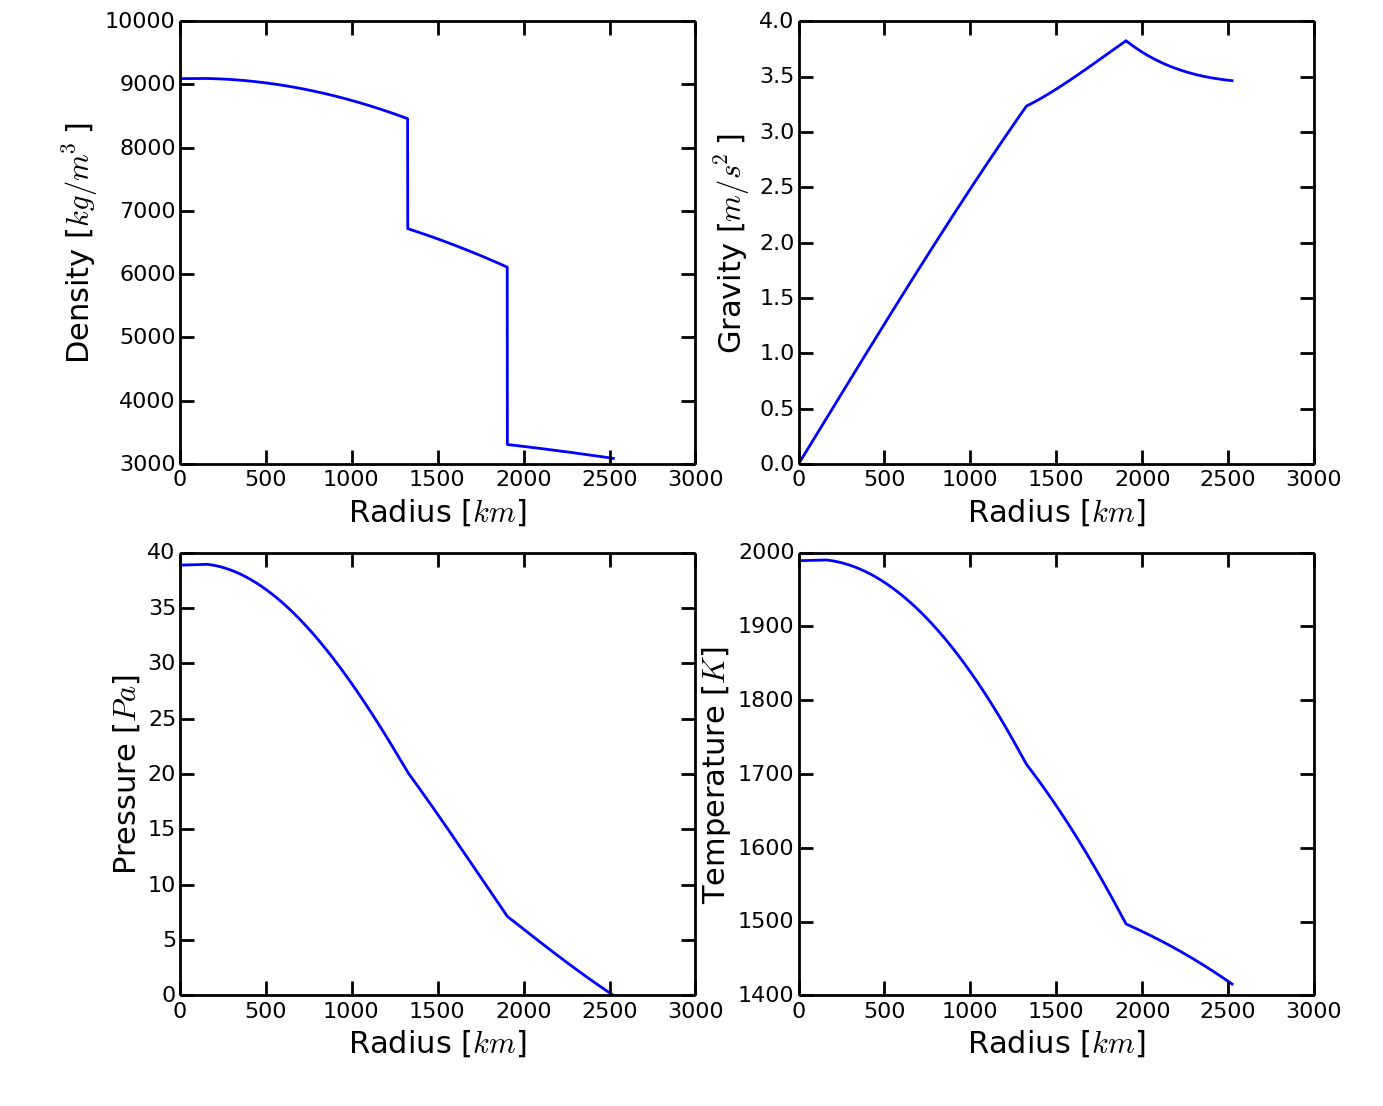
\includegraphics[width=0.15\textwidth]{profiles.png} &
 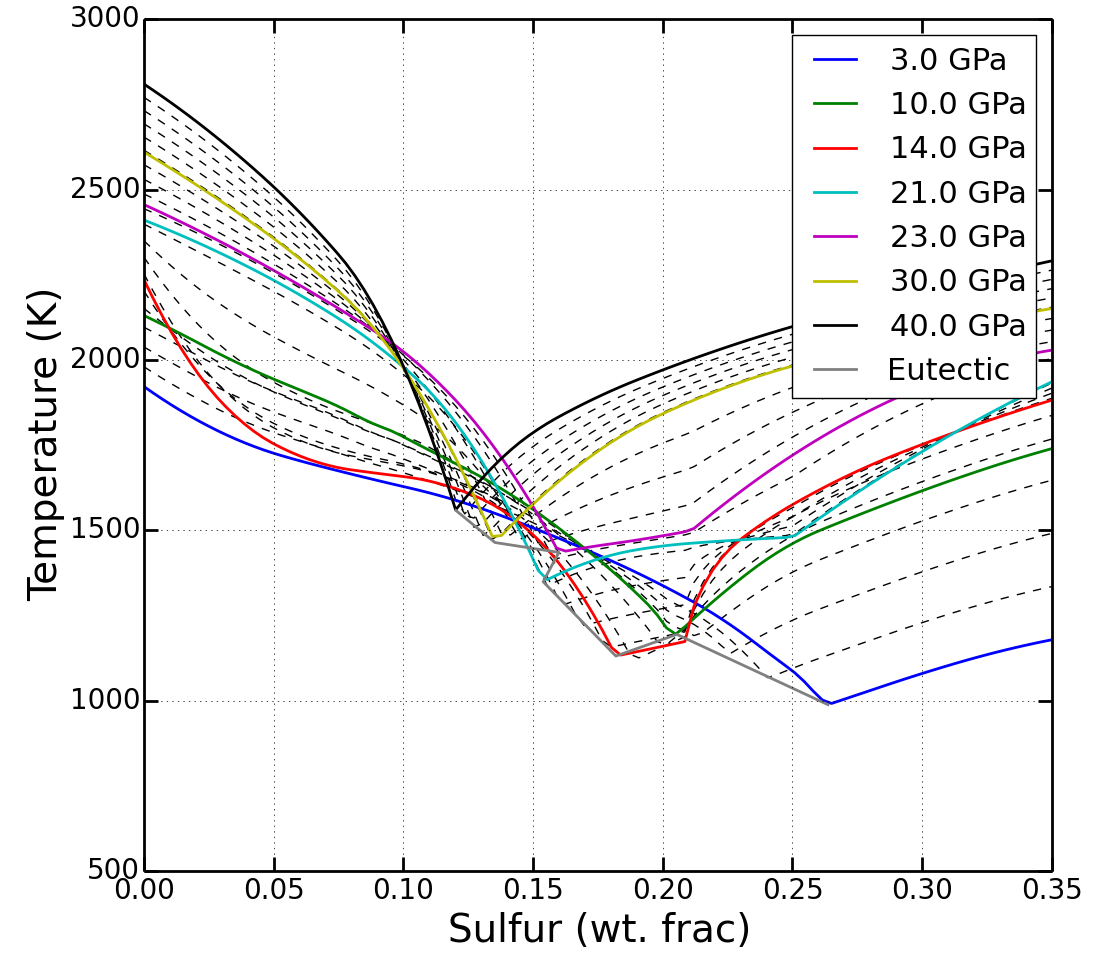
\includegraphics[width=0.15\textwidth]{Liquidus_model.png} \\
 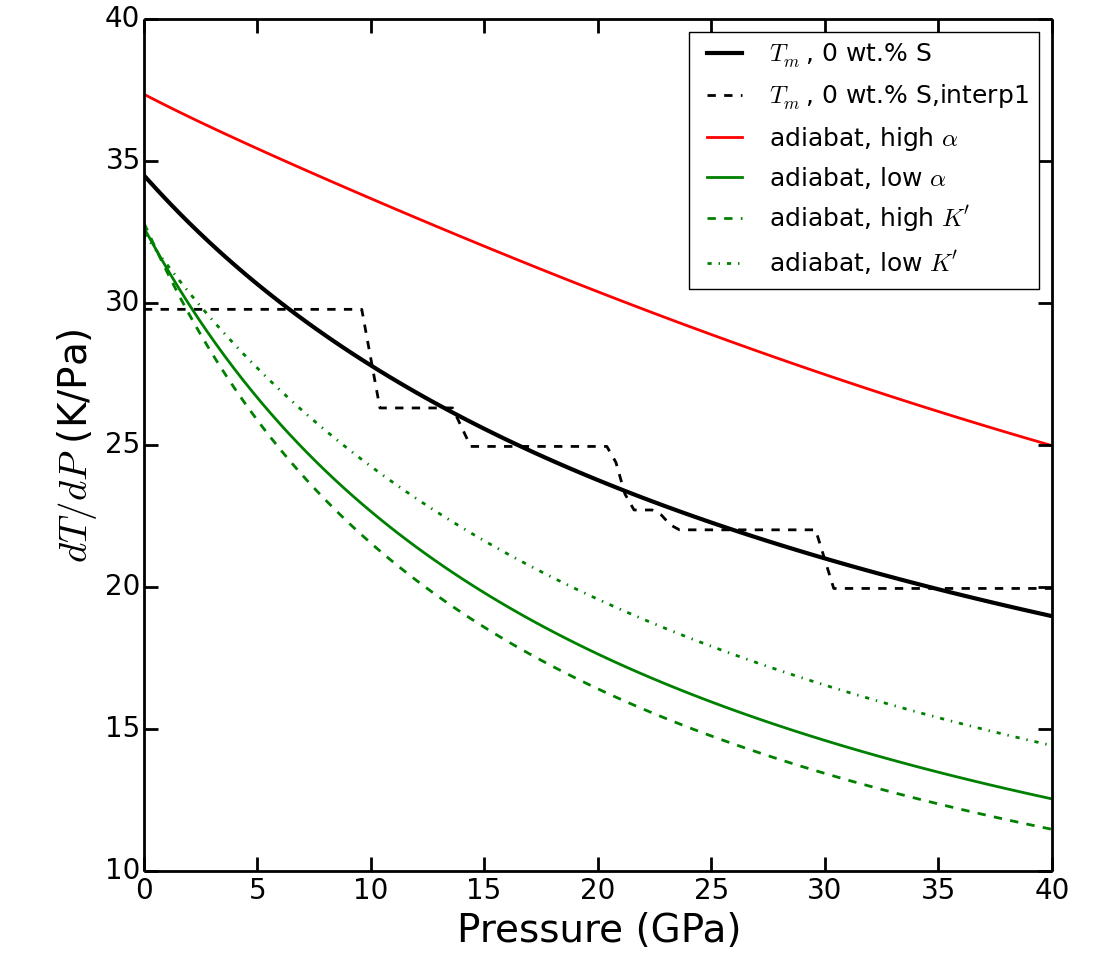
\includegraphics[width=0.15\textwidth]{clapeyron_1.png} &
 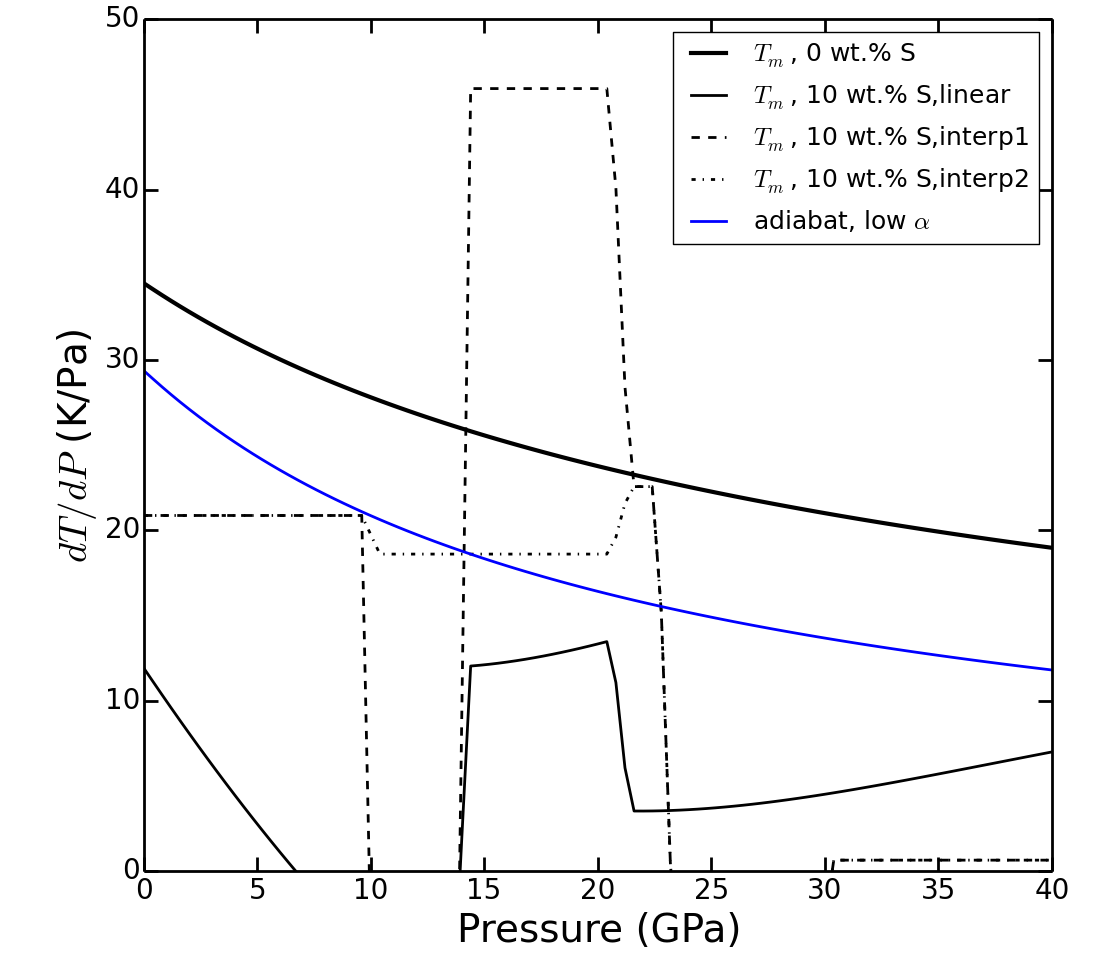
\includegraphics[width=0.15\textwidth]{clapeyron_2.png} \\
\end{tabular}
\captionof{figure}{ }
\label{interior_model}
\end{center}

\columnbreak

\section*{Parameterized convection and thermal evolution}



\section*{Speculative seismology}

In the future it may be possible to install one, or even a network of seismometers on Mercury. Would we be able to distingiush between different models of Mercury's interior? We extract self-consistent velocity and density models corresponding to two reasonable models (Dumberry and Rivoldini, 2014): one with 6 wt.\% sulfur in the core, corresponding to a 650km inner core, and 9 wt.\% sulfer in the core, with a 1325km inner core.
Raypaths and normal mode frequencies and eigenfunctions for these models are calculated using TauP Toolkit (Crotwell et al 1999) and Mineos (http://www.geodynamics.org) using Earth-like attenuation (Dziewonski \&  Anderson, 1981). The P-wave raypaths show that a P-wave shadow zones would not exist for the larger inner core. Differences in the inner core size also cause changes in the frequency and eigenfunctions of the normal modes. 

\begin{center}
\begin{tabular}{ccc}
 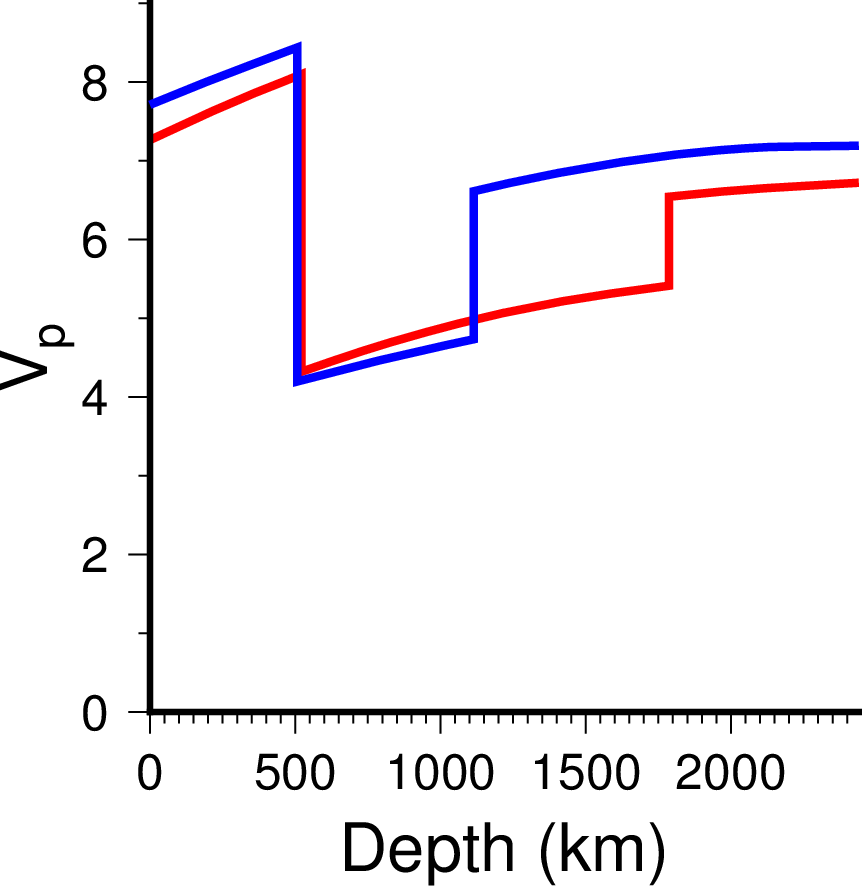
\includegraphics[width=0.09\textwidth]{merc_both_models_1} &
 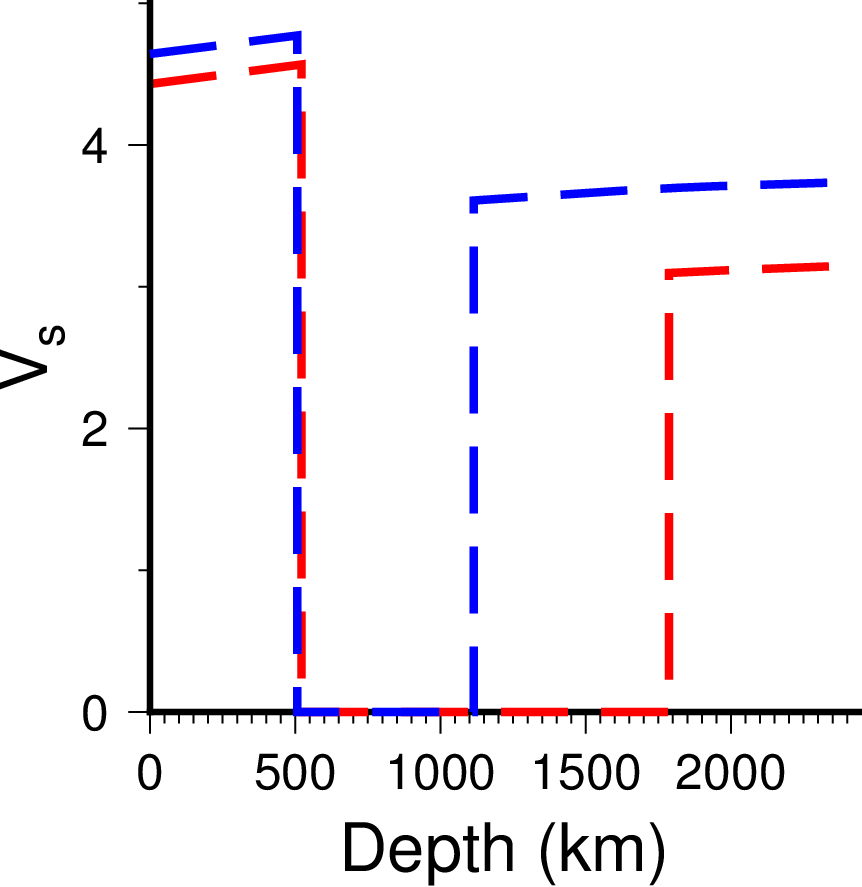
\includegraphics[width=0.09\textwidth]{merc_both_models_2} &
 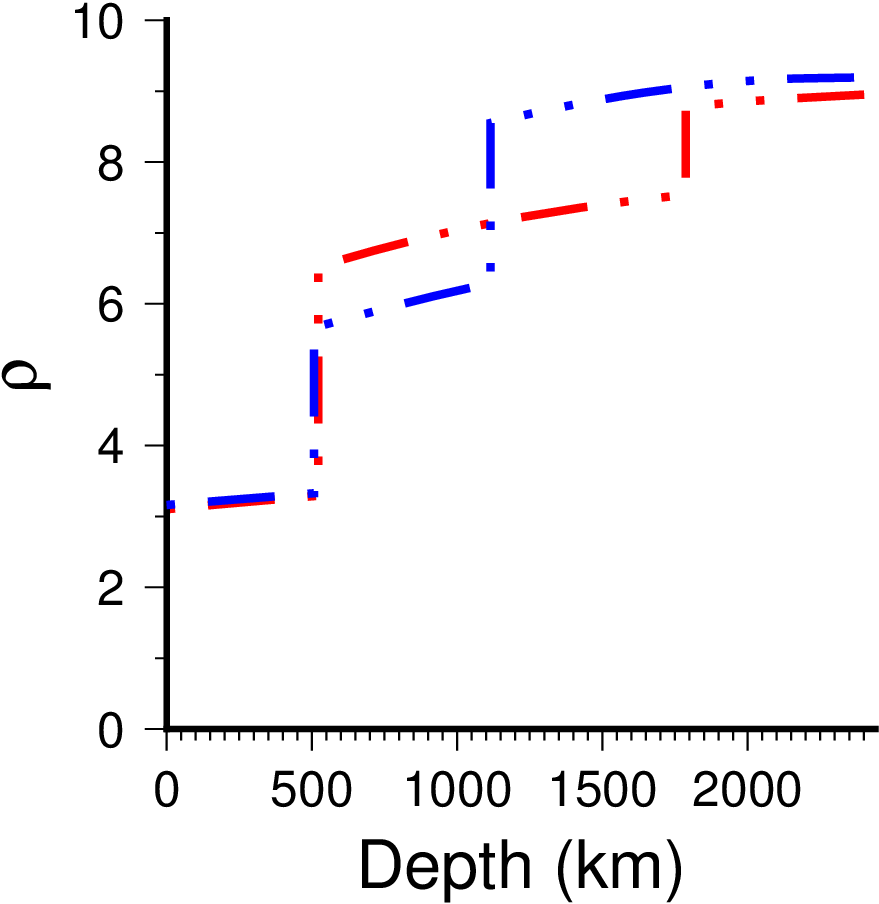
\includegraphics[width=0.09\textwidth]{merc_both_models_3} 
\end{tabular}
\captionof{figure}{  V$_p$, V$_s$ and $\rho$ profiles for two realisations of Mercury's interior. Red lines corespond to the smaller inner core and blue to the larger inner core.}
\end{center}

\columnbreak

\begin{center}
\begin{tabular}{ccc}
 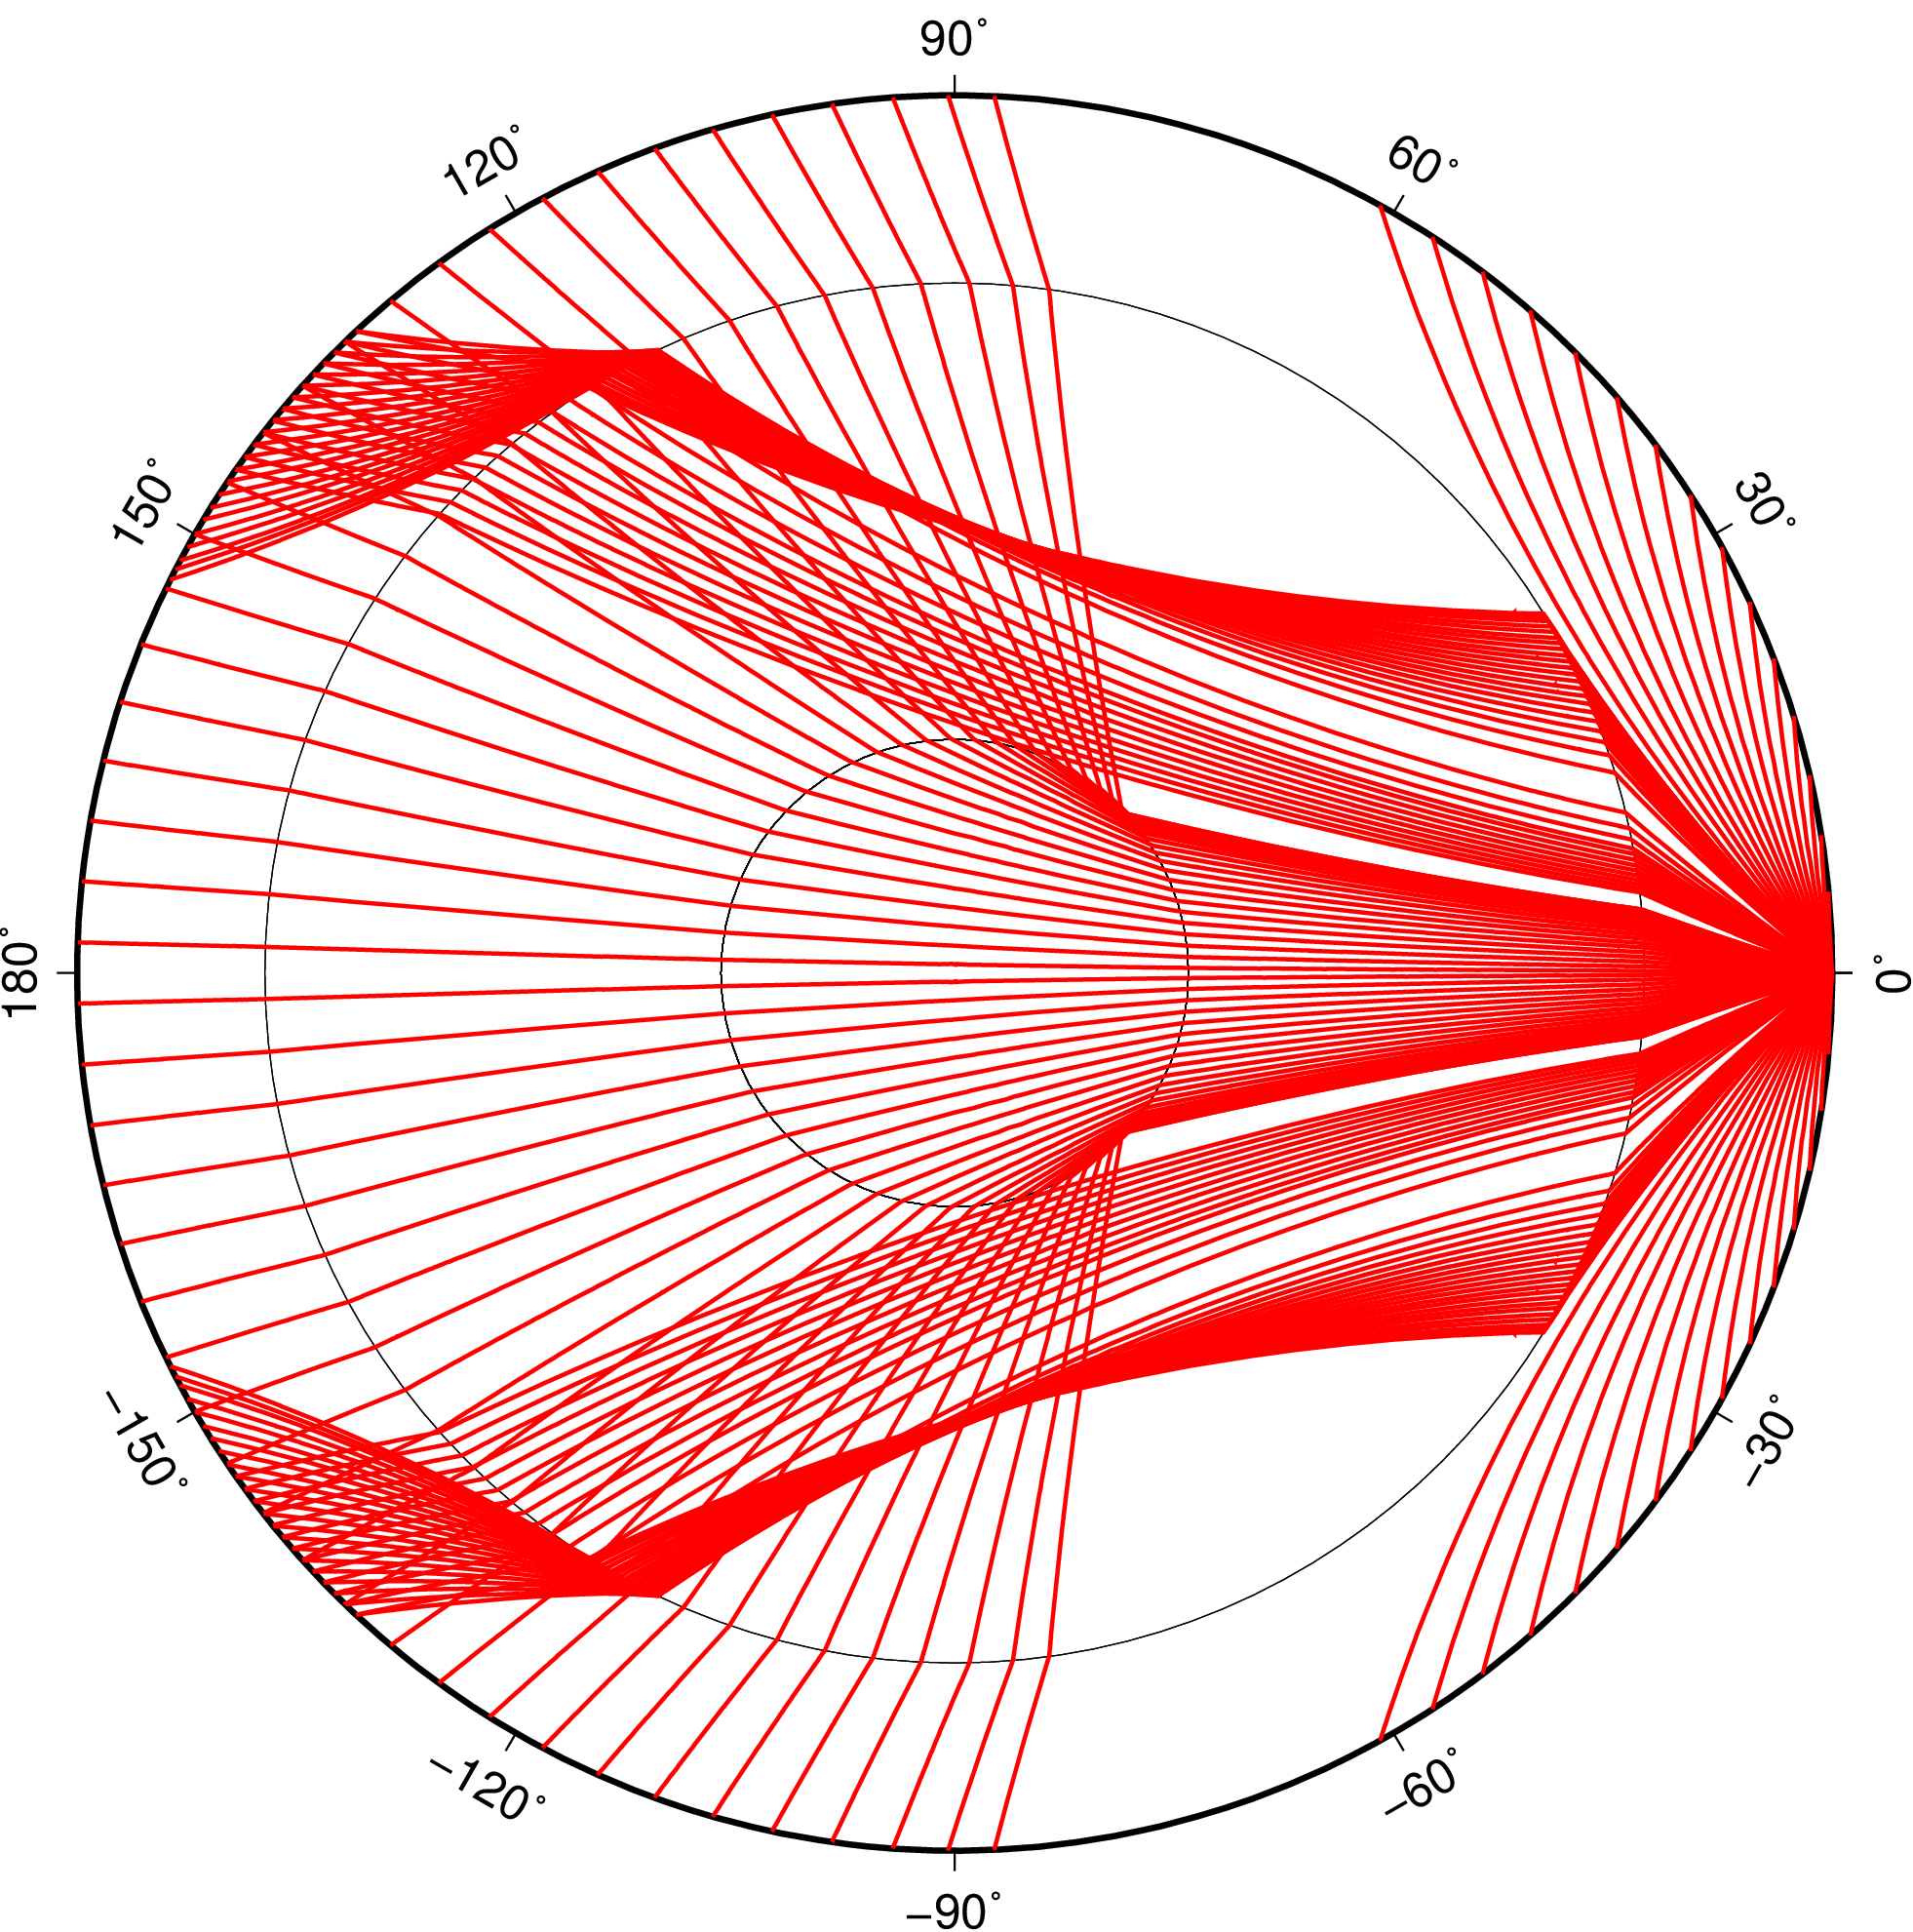
\includegraphics[width=0.12\textwidth]{smapath.png} &
 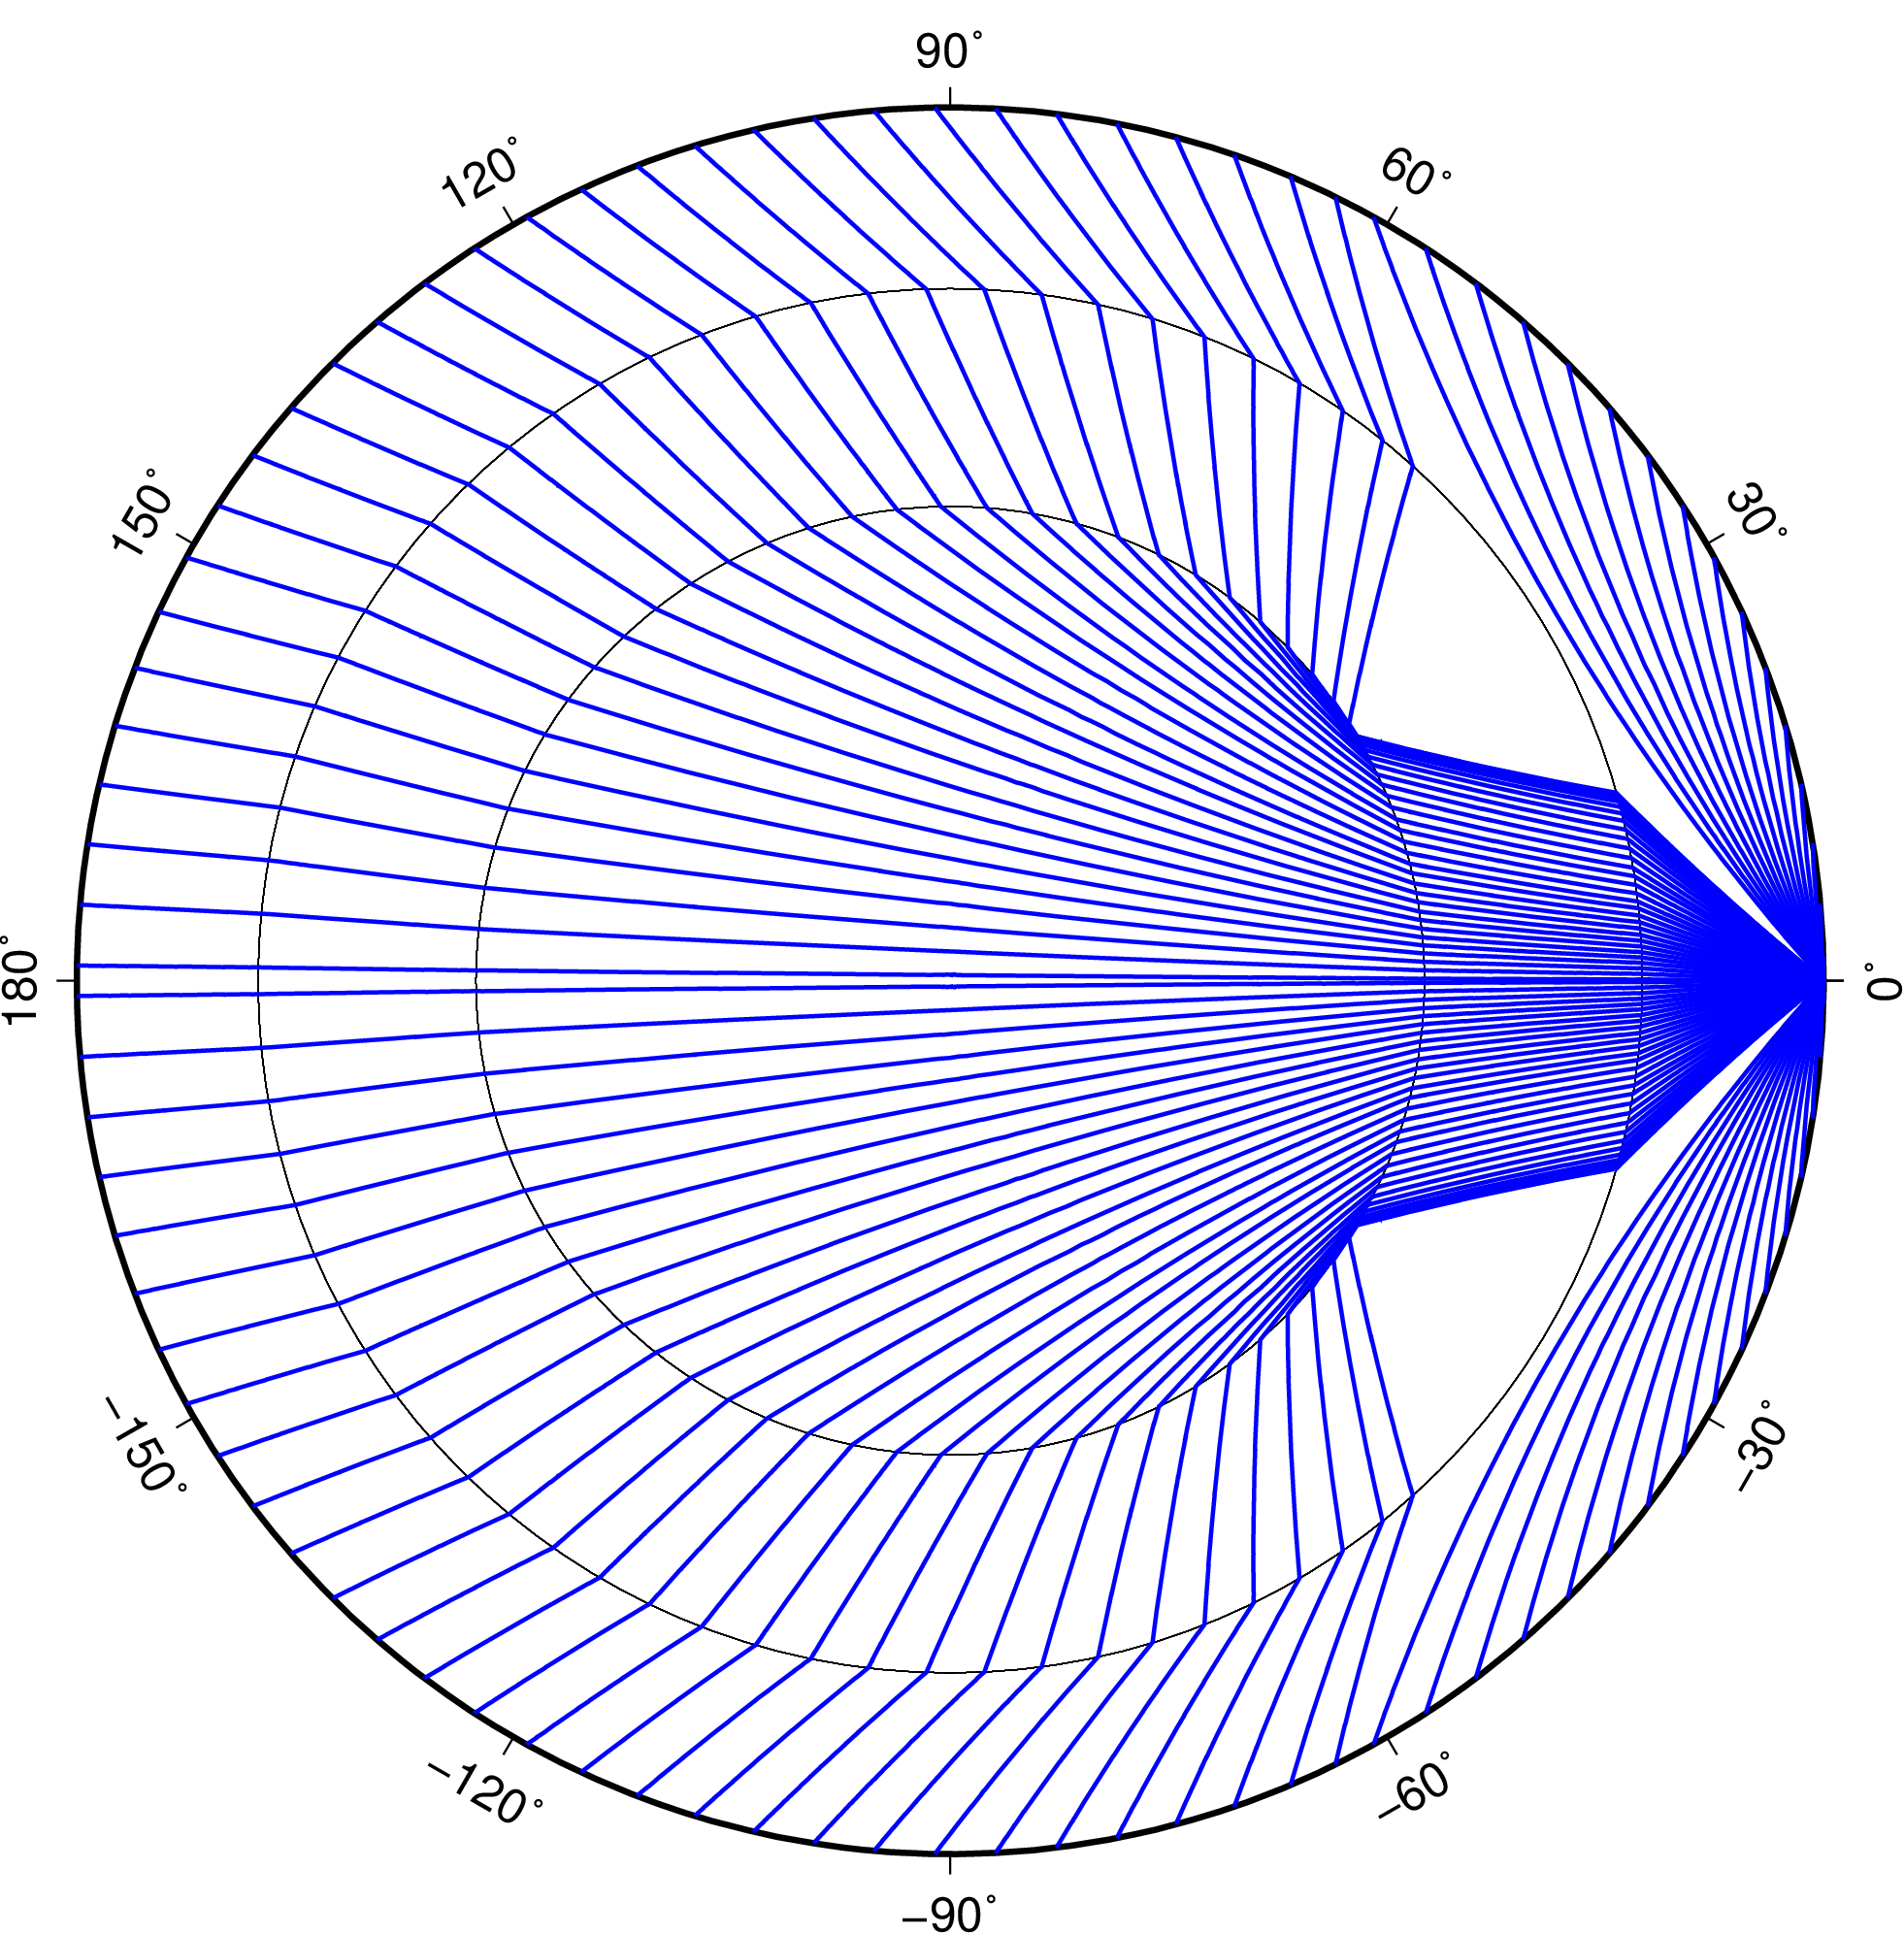
\includegraphics[width=0.12\textwidth]{bigpath.png} &
\end{tabular}
\captionof{figure}{  P, PKP and PKIKP paths for the two velocity models. }
\end{center}

A bigger impact on any future seismic observations of Mercury will be the presence of an FeS layer at the top of core, we plan to investiagte this in the future.



\section*{Dynamo simulation}

Mercury's unusual 3:2 spin-orbit resonance causes persistent temperature variations at the surface.  This boundary condition may create significant heat-flux variations at the CMB, especially if the mantle is not convecting.  Here we solve a simple conduction equation in the mercurian mantle to calculate an estimate of heat flux at the CMB.  This heat-flux variation is then used to inform the boundary conditions of a dynamo simulation using the \texttt{Calypso} code.
\\
We model a thermally driven dynamo in a rotating spherical shell with $r_{i}/r_{o} = 0.35$ (i.e.  $r_i$ = 700km).  The dynamo is driven with a non-dimensional heat flux $\mathrm{Nu} \sim 5$.  We test three cases for the heat-flux boundary condition: (1) homogeneous heat flux, (2) variations in the heat flux are scaled to be the same as the conducting-mantle variations, and (3) the variations in heat flux are scaled to be the ten times the conducting-mantle variations.
\begin{center}
\begin{tabular}{ccc}
 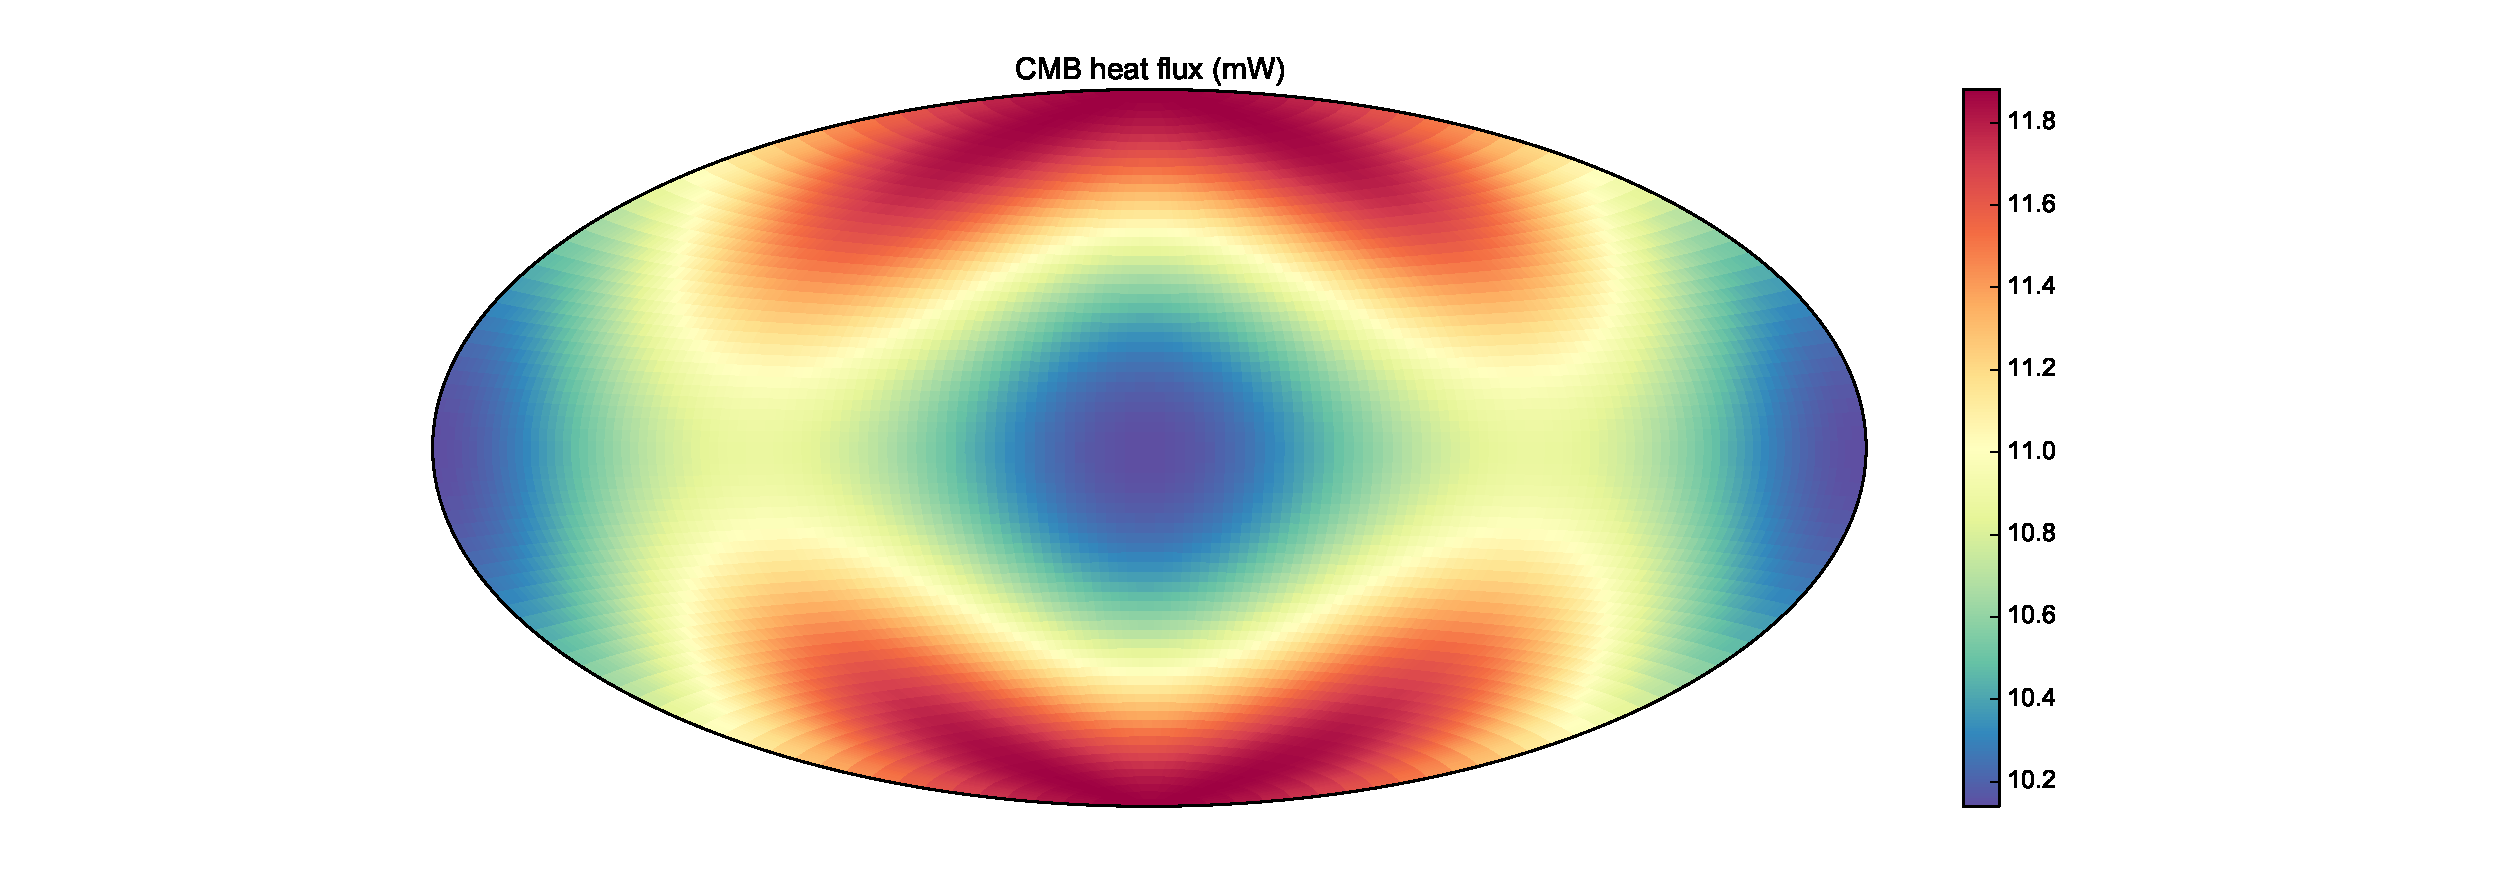
\includegraphics[width=0.14\textwidth]{CMB_flux.pdf} &
 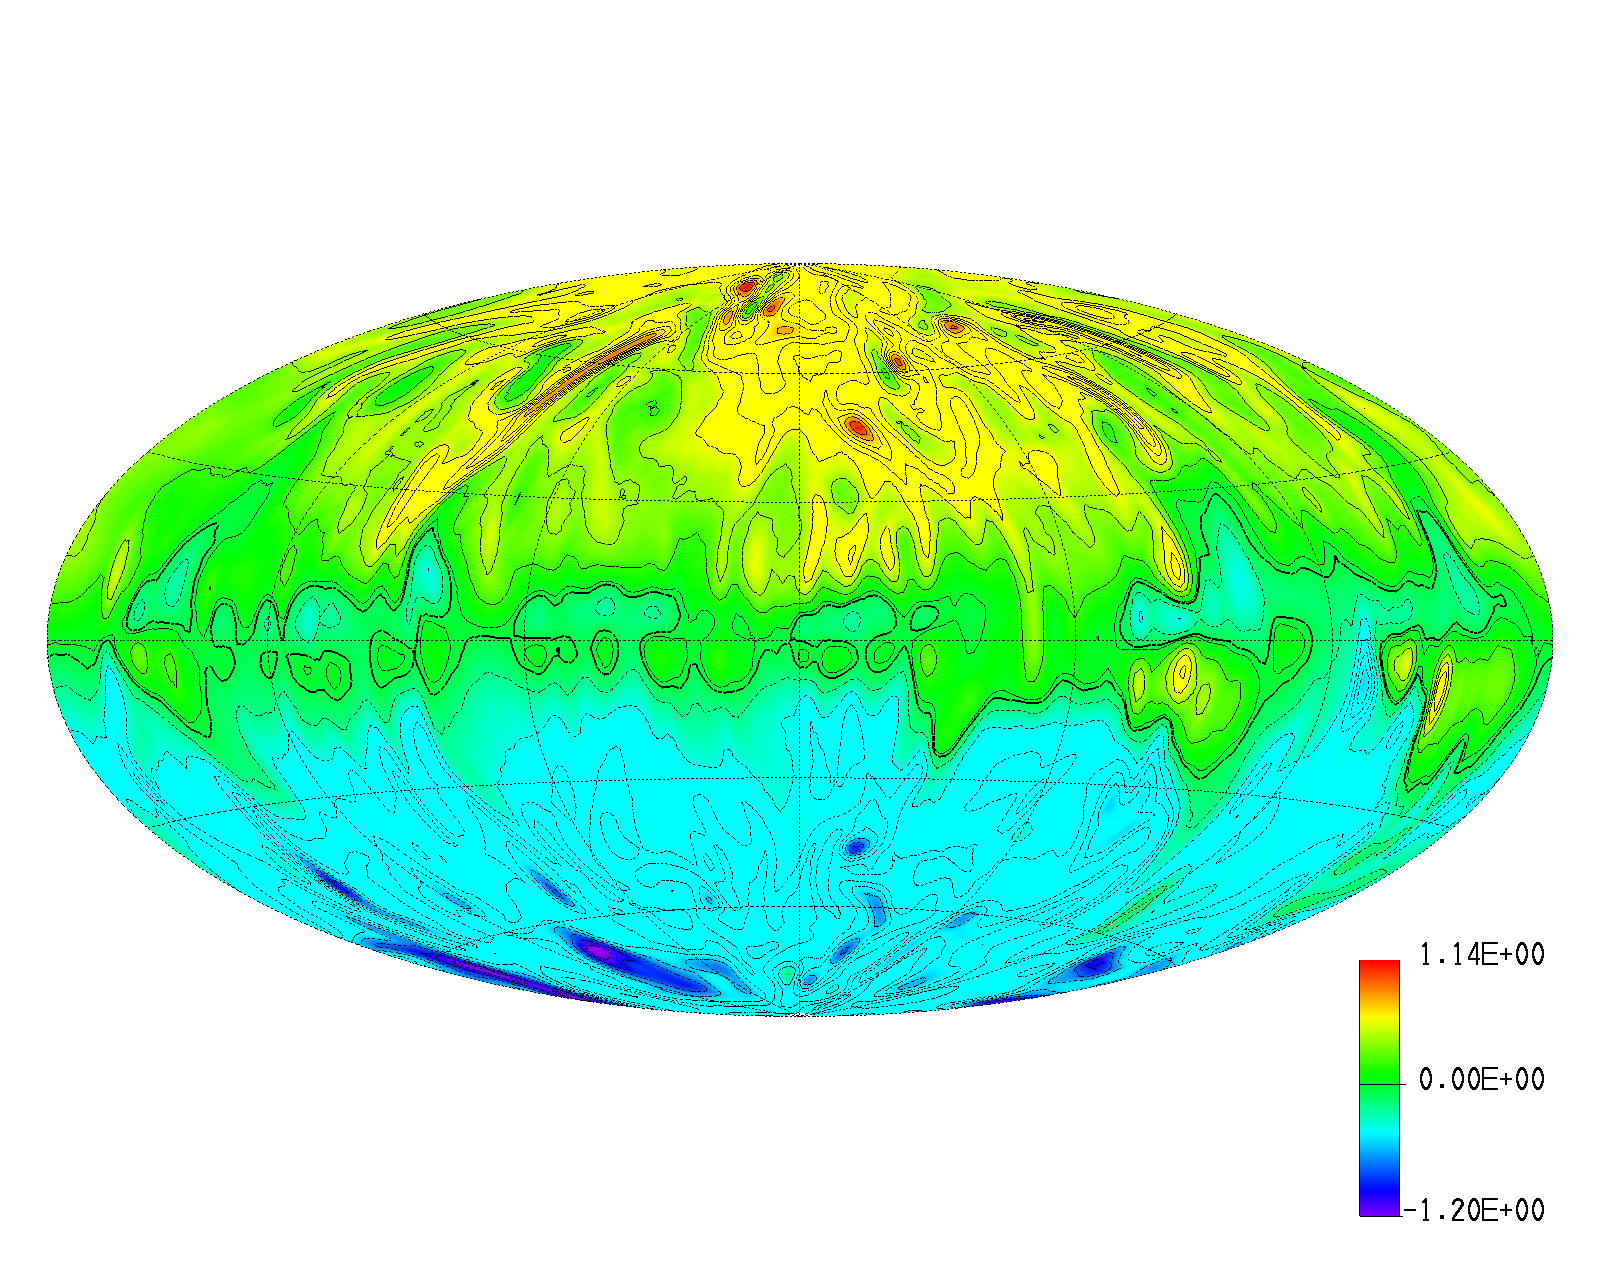
\includegraphics[width=0.08\textwidth]{br_cmb_x0.png} &
 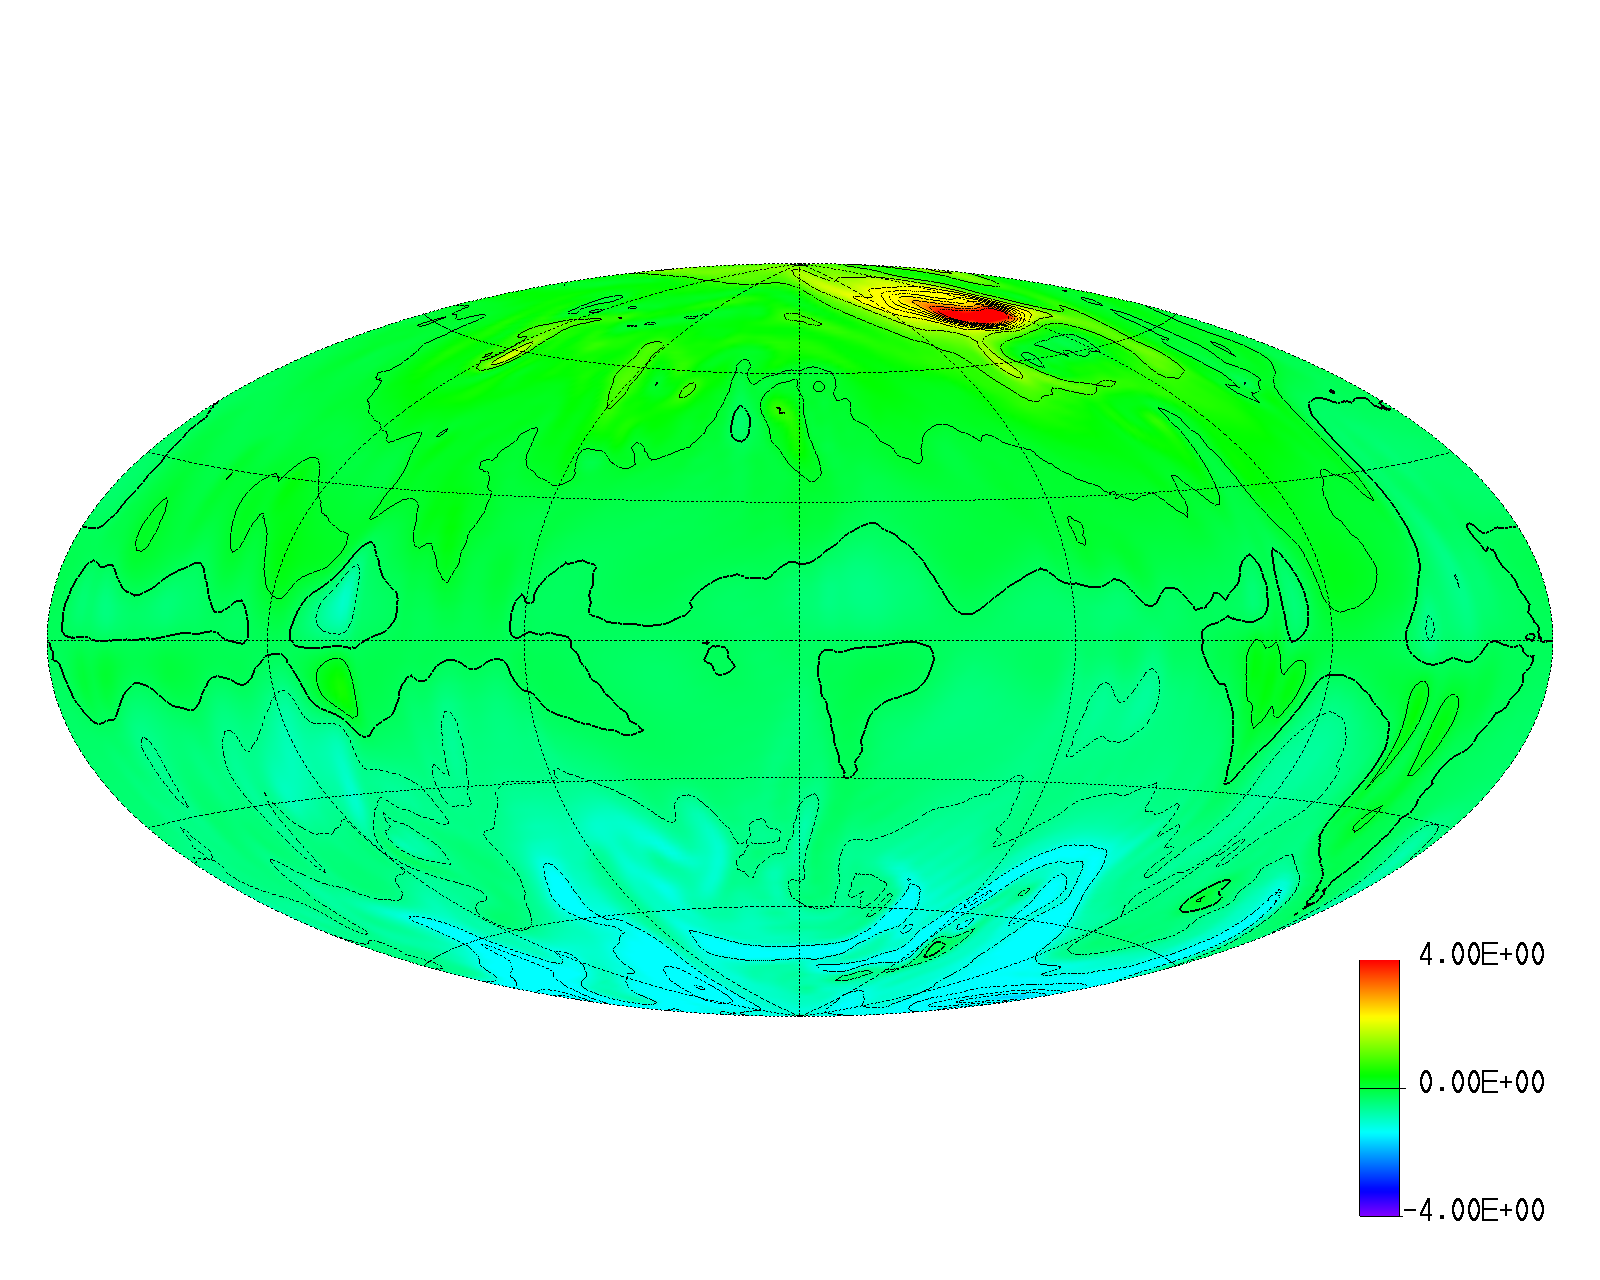
\includegraphics[width=0.08\textwidth]{br_cmb_x10.png}
\end{tabular}
\captionof{figure}{ Left: reat flux variations for a conducting mantle with negligible internal heating. The total CMB heat flux is $\sim 0.6 \mathrm{TW}$, and peak-to-peak variations are about 20\%. Right: radial magnetic field at the CMB for the case of ten times larger heat flux heterogeneity case (case 3). Center: radial magnetic field in the homogeneous heat flux case (case 1).
 }
\label{dynamo}
\end{center}

To summarize preliminary results from our dynamo simulations:
\begin{itemize}
\item Large heat fluxes at the poles induce intense magnetic fields inside of tangent cylinder.
\item This magnetic patch is not stable in the present parameter regime.
\item The obtained magnetic field is larger than that  the homogeneous heat flux case in the dipolar regime. The present solution may be too strong to explain the mercury's magnetic field. We need to test more cases .
\end{itemize}

{ \large References \\ \small
A. M. Dziewonski and D. L. Anderson: Preliminary reference Earth model. Phys. Earth Planet. Int. 25, 297–356 (1981).
H. P. Crotwell, T. J. Owens, and J. Ritsema. The TauP Toolkit: Flexible Seismic Travel-time and Ray-path Utilities. Seismol. Res. Lett., 70(2), 154–160 (1999). 
M. Dumberry and A. Rivoldini, Mercury’s inner core size and core-crystallization regime, Icarus, 248, 254-268 (2015).
 }
\\
{ \large Acknowledgements \\ \small
This project was initiated at the 2014 CIDER summer program.  We are grateful for continuing support from CIDER- NSF: 1135452.
Data for the Fe-FeS liquidus model was compiled and interpolated by June Wick and Nick Knezek.
We are grateful for helpful discussions with Bruce Buffett, Chris Davies, Mathieu Dumberry, and numerous CIDER participants.
}

\end{multicols}


\end{document}

